%!TEX program = lualatex
% Arquivo: Template_Estat_Texto.tex

\documentclass[a4paper,12pt]{article}

% =========================================================
% Idioma e tipografia (LuaLaTeX)
% =========================================================
\usepackage[portuguese]{babel}
\usepackage{fontspec}
\setmainfont{Latin Modern Roman}

% =========================================================
% Layout
% =========================================================
\usepackage[top=3cm,bottom=2.5cm,left=3cm,right=2.5cm]{geometry}
\usepackage{setspace}
\onehalfspacing
\usepackage{indentfirst}
\setlength{\parindent}{1.25cm}

% =========================================================
% Matemática (align*, etc.)
% =========================================================
\usepackage{amsmath}
\usepackage{amssymb}

% =========================================================
% Tabelas, listas, figuras
% =========================================================
\usepackage{booktabs}
\usepackage{array}
\usepackage{enumitem}
\setlist[itemize]{noitemsep,topsep=3pt}
\setlist[enumerate]{noitemsep,topsep=3pt}

\usepackage{graphicx}
\usepackage{float}
\usepackage{pdflscape}
\graphicspath{{./}{./imagens/}{./figuras/}}

% =========================================================
% Links
% =========================================================
\usepackage{hyperref}
\usepackage{xurl}
\hypersetup{
  colorlinks=true,
  linkcolor=black,
  urlcolor=blue,
  citecolor=black,
  pdfauthor={},
  pdftitle={}
}

% =========================================================
% Texto de preenchimento (lorem)
% =========================================================
\usepackage{lipsum}

% =========================================================
% Dados da capa
% =========================================================
\newcommand{\Instituicao}{Universidade / Instituição}
\newcommand{\Curso}{Disciplina / Curso}
\newcommand{\Professor}{Professor: Nome Sobrenome}
\newcommand{\Aluno}{Aluno: José Mauro Xavier Elsas}
\newcommand{\Cidade}{Rio de Janeiro}
\newcommand{\Ano}{2026}

\title{\textbf{Título do Documento}}
\author{\Aluno}
\date{\Cidade --- \Ano}

\begin{document}

% =========================================================
% Capa (página de rosto)
% =========================================================
\begin{titlepage}
\centering
{\large \Instituicao \par}
\vspace{0.5cm}
{\large \Curso \par}
\vspace{1.0cm}

{\LARGE \textbf{Título do Documento} \par}
\vspace{0.6cm}
{\Large Subtítulo (opcional) \par}

\begin{figure}[H]
  \centering
  
\includegraphics[width=.3\linewidth]{./uerj.jpg}
\end{figure}

\vfill



\begin{flushright}
\Aluno\\
\Professor
\end{flushright}

\vspace{1.0cm}
{\Cidade --- \Ano \par}
\end{titlepage}

% =========================================================
% Sumário
% =========================================================
\tableofcontents
\newpage

% =========================================================
% Corpo do texto (exemplos)
% =========================================================
\section{Introdução}

\section{Determinação do Vetor Médio de Corrente}

Os dados de corrente foram obtidos a partir do sistema SiMCosta, provenientes de um correntômetro acústico Doppler (ADCP) instalado na região de Linhares (ES), próximo à desembocadura do Rio Doce.

A base de dados consiste em uma série temporal com resolução aproximada de 30 minutos, contendo medições de direção e magnitude da corrente para 25 células ao longo da coluna d'água.

\subsection{Pré-processamento}

Os dados foram importados em ambiente Python utilizando a biblioteca \texttt{pandas}, com remoção das linhas de metadados e reconstrução da variável temporal a partir dos campos de data e hora.

A inspeção inicial indicou:
\begin{itemize}
    \item consistência temporal da série;
    \item ausência de valores faltantes;
    \item adequação estrutural para análise vetorial.
\end{itemize}

\subsection{Metodologia}

As direções de corrente, fornecidas em graus azimutais, foram interpretadas como a direção \textbf{para onde} a corrente se desloca.

Para evitar inconsistências associadas à média direta de ângulos, foi adotada uma abordagem de \textbf{soma vetorial}, com decomposição das velocidades em componentes:

\begin{equation}
u = V \cdot \sin(\theta)
\end{equation}

\begin{equation}
v = V \cdot \cos(\theta)
\end{equation}

onde $u$ e $v$ representam, respectivamente, as componentes zonal (leste-oeste) e meridional (norte-sul).

Os valores extremos foram tratados por meio de um filtro baseado no percentil 99 da magnitude para cada célula, removendo apenas outliers associados a ruído instrumental. A comparação entre resultados com e sem filtragem indicou impacto inferior a 5\%, garantindo a robustez da análise.

\subsection{Resultados por Célula}

Foram analisadas as células 001 a 010, representativas da porção superior da coluna d'água.

\begin{table}[H]
\centering
\begin{tabular}{cccc}
\toprule
Célula & Direção (°) & Velocidade (mm/s) & Observação \\
\midrule
001 & 182.8 & 106.7 & Superfície \\
002 & 188.1 & 154.2 &  \\
003 & 190.5 & 194.7 &  \\
004 & 192.6 & 204.2 & Máximo \\
005 & 194.5 & 200.6 &  \\
006 & 196.0 & 186.7 &  \\
007 & 198.4 & 173.7 &  \\
008 & 201.0 & 160.9 &  \\
009 & 203.0 & 144.4 &  \\
010 & 205.2 & 130.0 &  \\
\bottomrule
\end{tabular}
\caption{Vetor médio por célula (após filtragem p99).}
\end{table}

\subsection{Vetor Médio Representativo}

A média vetorial conjunta das células 001 a 010 resultou em:

\begin{itemize}
    \item Componente zonal média: $u \approx -43.3$ mm/s
    \item Componente meridional média: $v \approx -158.9$ mm/s
    \item Velocidade média: $\approx 0{,}16$ m/s
    \item Direção média: $\approx 195^\circ$
\end{itemize}

\subsection{Interpretação}

Os resultados indicam uma corrente predominante no sentido sul a sul-sudoeste, com leve componente para oeste.

Observa-se uma rotação progressiva da direção com a profundidade, partindo de aproximadamente $180^\circ$ nas camadas mais superficiais e atingindo cerca de $205^\circ$ nas camadas mais profundas analisadas.

Esse padrão é consistente com a circulação costeira regional, caracterizada por escoamento predominantemente paralelo à linha de costa.

A utilização dos dados de Linhares como proxy regional para o litoral norte fluminense é justificada pela similaridade geométrica da costa e pela coerência com a deriva litorânea observada na região.

Segue gráfico da leitura da direção da correnteza em função da profundidade.

\begin{figure}
    \centering
    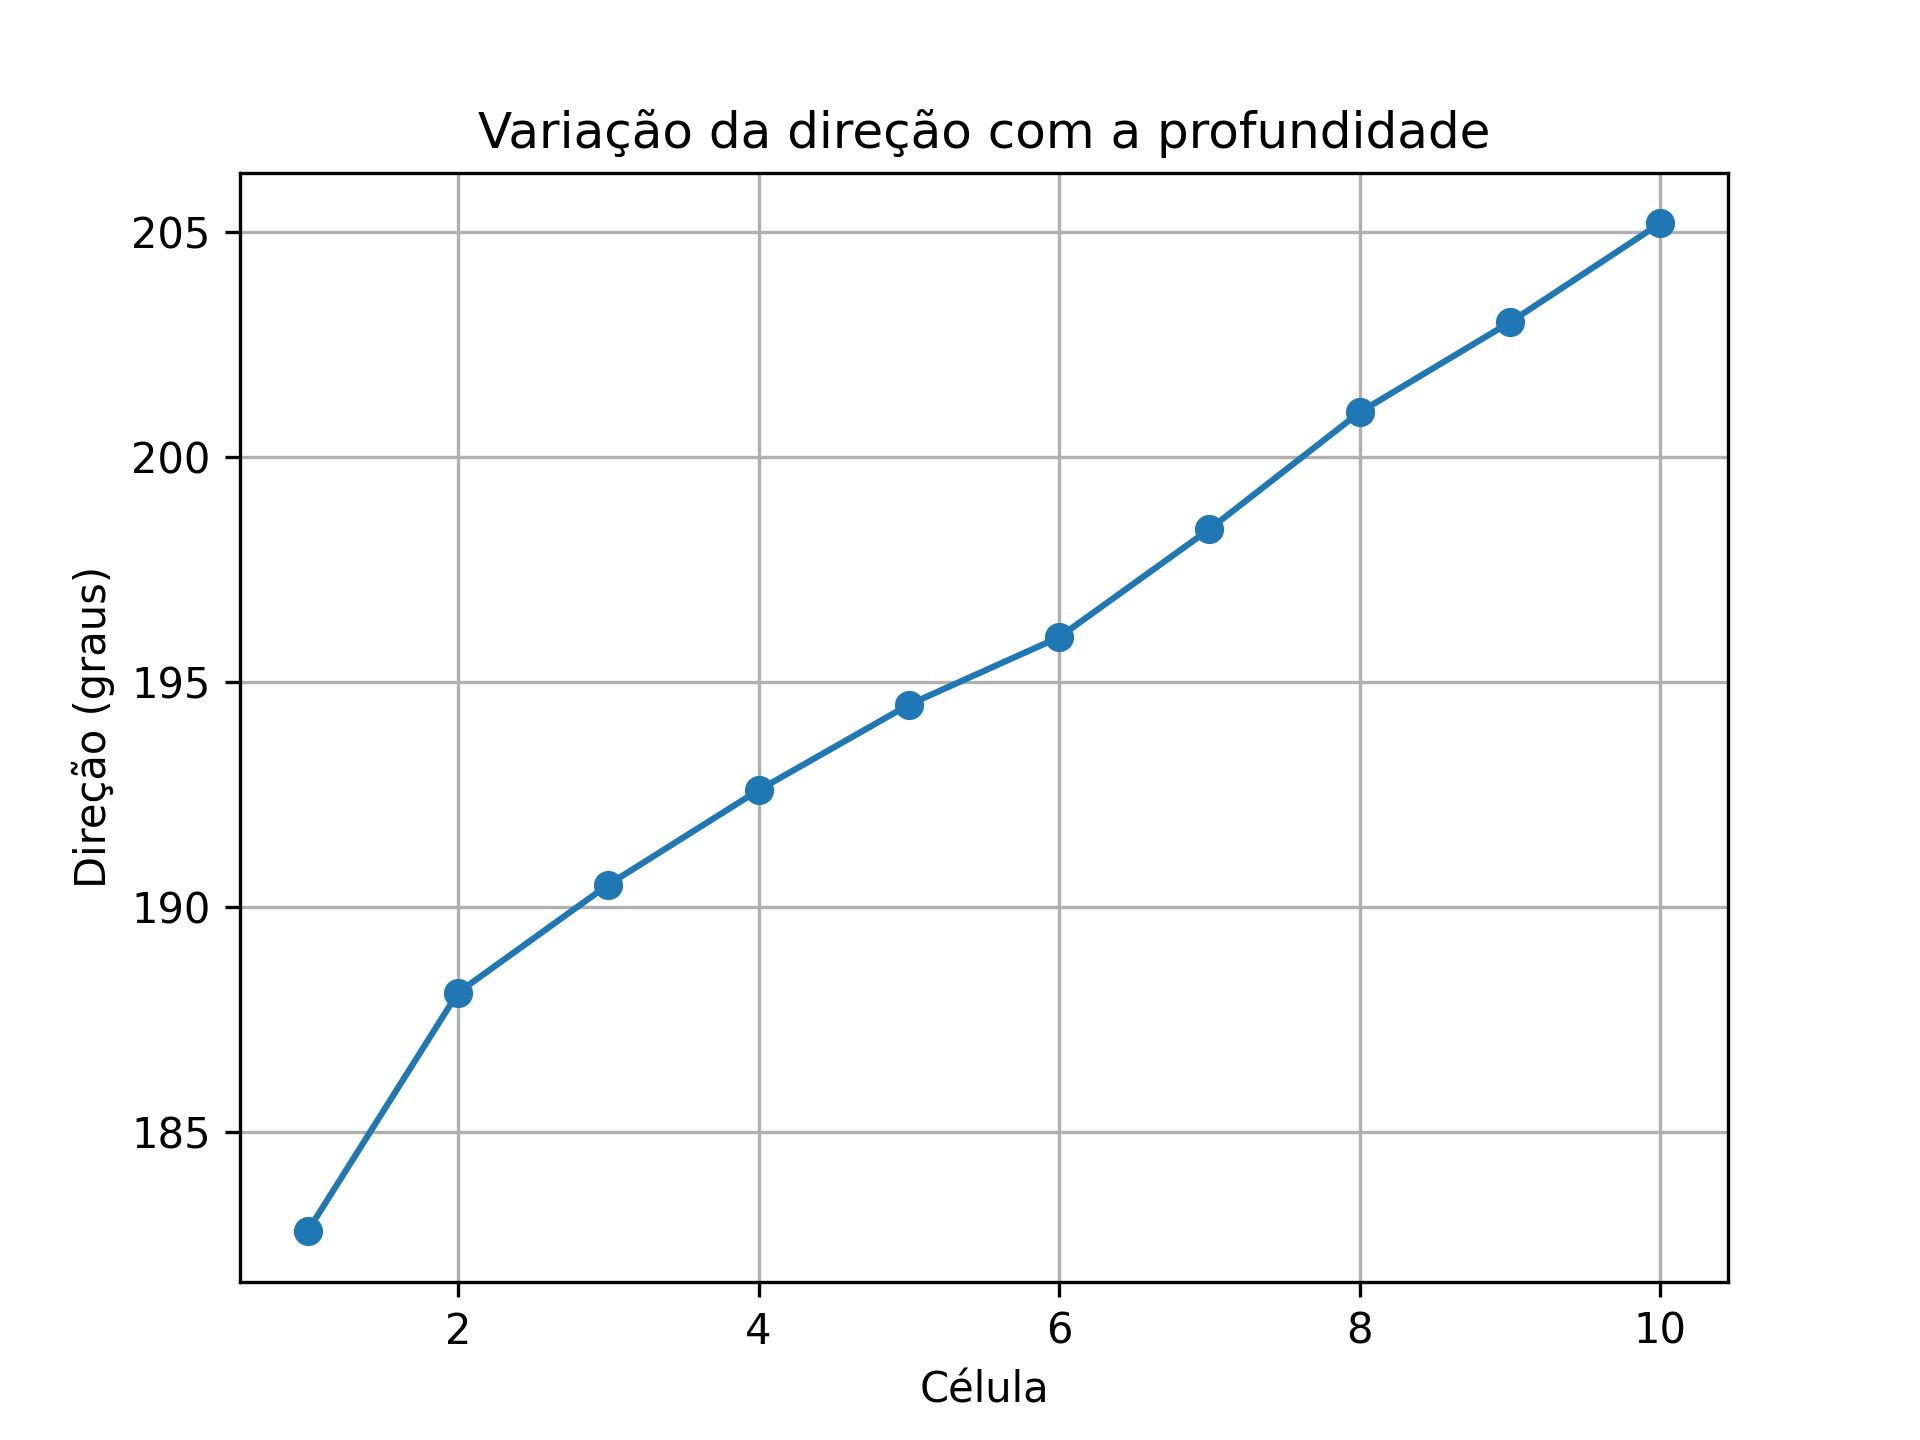
\includegraphics[width=.9\linewidth]{direcao_cells.png}
\end{figure}

% =========================================================
% Referências (entra no sumário)
% =========================================================
\newpage
\phantomsection
\addcontentsline{toc}{section}{Referências}
\begin{thebibliography}{99}

\bibitem{exemplo1}
SOBRENOME, Nome.
\textbf{Título do livro}.
Cidade: Editora, 2020.

\bibitem{exemplo2}
AUTOR, Nome.
Título do artigo.
\textit{Nome do Periódico}, v. 10, n. 2, p. 1--20, 2021.
Disponível em: \url{https://exemplo.com}. Acesso em: 30 jan. 2026.

\end{thebibliography}

\end{document}
